\subsubsection*{Variables}
For the relativistic notation in Chapter~\ref{ch:furry_pic}, the symbols $x$, $y$, $z$, $z_1$, $z_2$, and $p$ are used for four vectors corresponding to $x^\mu=(x^0,\mathbf{x})=(x^0,x^1,x^2,x^3)$, where bold symbols stand for the three-component spacial vectors. The scalar product is $x_\mu y^\mu = x^0 y^0 - \mathbf{x}\cdot\mathbf{y}$, corresponding to the metric $g^{\mu\nu}=\text{diag}(1,-1,-1,-1)$.\\
In all other chapters, three dimensional vectors in spherical coordinates are written as bold symbols $\mathbf{r}=(r,\vartheta,\varphi)$, where $\varphi$ is the polar angle and $\vartheta$ is the azimuthal angle. The volume element is as usual $\text{d}^3\mathbf{r}=\text{d}r\text{d}\varphi\text{d}\vartheta\, r^2 \sin\vartheta $.
\subsubsection*{Feynman rules}
In Chapter~\ref{ch:furry_pic}, the following Feynman rules in position space are needed, where the notation follows~\cite{itzykson2005}. If external lines are involved, the corresponding solutions of the Dirac equation have to be used.\\

\begin{tabular}{lll}
fermion propagator (ext. field):&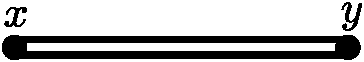
\includegraphics[width=0.2\linewidth]{pics/feynrule_1.pdf} & $S_{\mathcal{A}}(x,y)\phantom{-}$ from Eq.~\eqref{eq:extpropdef}\\[7pt]
fermion propagator (free):&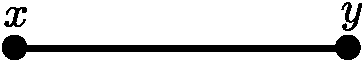
\includegraphics[width=0.2\linewidth]{pics/feynrule_2.pdf} &$S_{F}(x-y)$ from Eq.~\eqref{eq:freepropdef}\\[7pt]
photon propagator:\vspace{-7pt}&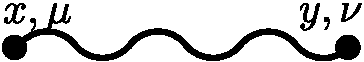
\includegraphics[width=0.2\linewidth]{pics/feynrule_3.pdf} &$g_{\mu\nu}\cfrac{1}{4\pi^2}\cfrac{1}{(x-y)^2-i\epsilon}$\\
(in Feynman gauge)\vspace{-7pt}\\
vertex:&
\includegraphics[width=0.2\linewidth]{pics/feynrule_4.pdf} &$-ie\gamma^\mu\int\text{d}^4x$
\end{tabular}
\subsubsection*{Dirac matrices}
The following representation of the Dirac matrices is chosen, following~\cite{greiner2000}:\\
\textit{$\beta$ and $\gamma$ matrices:}\\[-10pt]
\begin{equation}
\beta=\gamma^0 =
\begin{pmatrix}
\boldsymbol{1}&\boldsymbol{0}\\
\boldsymbol{0}&\boldsymbol{-1}
\end{pmatrix};\qquad
\gamma^{i} = 
\begin{pmatrix}
\boldsymbol{0}&\boldsymbol{\sigma}^i\\
-\boldsymbol{\sigma}^i&\boldsymbol{0}
\end{pmatrix}
\end{equation}
with\\[-10pt]
\begin{equation}
\boldsymbol{0}=
\begin{pmatrix}
0&0\\0&0
\end{pmatrix};\quad
\boldsymbol{1}=
\begin{pmatrix}
1&0\\0&1
\end{pmatrix};\quad
\boldsymbol{\sigma}^1=
\begin{pmatrix}
0&1\\1&0
\end{pmatrix};\quad
\boldsymbol{\sigma}^2=
\begin{pmatrix}
0&-i\\i&0
\end{pmatrix};\quad
\boldsymbol{\sigma}^3=
\begin{pmatrix}
1&0\\0&-1
\end{pmatrix};\quad
\end{equation}
\textit{$\alpha$ matrices:}
\begin{equation}
\boldsymbol{\alpha}^i = \gamma^0 \gamma^i =
\begin{pmatrix}
\boldsymbol{0}&\boldsymbol{\sigma}_i\\
\boldsymbol{\sigma}_i&\boldsymbol{0}
\end{pmatrix}
;\quad\text{with }i \in \{1,2,3\}.
\end{equation}
$\phantom{1}$

